\documentclass{article}
\usepackage{amsmath}
\usepackage[margin=1in]{geometry}
\usepackage{amsfonts}
\usepackage{hyperref}
\usepackage{graphicx}
\usepackage{amssymb}
\usepackage{wasysym}
\usepackage{cancel}

\begin{document}
	
	\title{Elementary Row Operations}
	\author{Andy Chong Sam}	
	\maketitle	
	
\section {The Three Operations}

\par \noindent Given a matrix that represents the coefficients in a linear system, the three operations are:

\begin{itemize}
  \item Exchange any two rows
  \item Multiply a row by a constant
  \item Add a multiple of one row to another row

\end{itemize}

\section {Graphical Intuition}

\par \noindent Elementary row operations can be applied to solve systems of linear equations. We will first consider a 2 variable example (which can be solved more easily with algebra) and a 3 variable example (where these operations become more useful):
\newline
\newline
\framebox{
	\parbox{\linewidth}{
	\par\noindent \textbf{Ex. 1} Find the point of intersection between \( y = 1 + 2x \) and \(y = 5-2x \)
	\par\noindent We will first rewrite these as \(-2x + y =1 \) and \(2x + y = 5 \) and fill in the matrix:
\newline

\[
\left(\begin{array}{@{}cc|c@{}}
	-2 & 1 & 1 \\
	&&\\
	2 & 1 & 5
\end{array}\right)
\xrightarrow[]{-R_1=R_1}
\left(\begin{array}{@{}cc|c@{}}
    2 & -1 & -1 \\
   &&\\
    2 & 1 & 5
\end{array}\right)
\xrightarrow[]{\frac{1}{2}R_2=R_2}
\left(\begin{array}{@{}cc|c@{}}
    2 & -1 & -1 \\
   &&\\
    1 & \frac{1}{2} & \frac{5}{2}
\end{array}\right)
\xrightarrow[]{R_1 - R_{2}=R_1}
\left(\begin{array}{@{}cc|c@{}}
    1 & -\frac{3}{2} & -\frac{7}{2} \\
    &&\\
    1 & \frac{1}{2} & \frac{5}{2}
\end{array}\right)
 \xrightarrow[]{R_2 - R_{1}=R_2}
\]

\[
\left(\begin{array}{@{}cc|c@{}}
	1 & \frac{1}{2} & \frac{5}{2} \\
	&&\\
	0 & 2 & 6
\end{array}\right)
 \xrightarrow[]{\frac{1}{2}R_2 = R_2}
 \left(\begin{array}{@{}cc|c@{}}
	1 & \frac{1}{2} & \frac{5}{2} \\
	&&\\
	0 & 1 & 3
\end{array}\right)
 \xrightarrow[]{R_1 - \frac{1}{2}R_2 = R_1} 
\left(\begin{array}{@{}cc|c@{}}
	1 & 0 & 1 \\
	&&\\
	0 & 1 & 3
\end{array}\right)
\]

\par\noindent \textbf{Solution:}  \( x=1, y =3\) . 
\\
	}
}
\newline
\newline
\newline
\framebox{
	\parbox{\linewidth}{
	\par\noindent \textbf{Ex. 2} Describe the intersection between \(2x + 3y - 4z = 3\) and \(x+6y-5z=8\).
\newline
\[
\left(\begin{array}{@{}ccc|c@{}}
	2 & 3 & -4 & 3 \\
	&&\\
	1 & 6 & -5 & 8
\end{array}\right)
 \xrightarrow[]{R_1 - R_2 = R_1}
 \left(\begin{array}{@{}ccc|c@{}}
	1 & -3 & 1 & -5 \\
	&&\\
	1 & 6 & -5 & 8
\end{array}\right)
\xrightarrow[]{R_2 - R_1 = R_2}
 \left(\begin{array}{@{}ccc|c@{}}
	1 & -3 & 1 & -5 \\
	&&\\
	0 & 9 & -6 & 13
\end{array}\right) 
\xrightarrow[]{\frac{1}{9}R_2 = R_2}
\]

\[
 \left(\begin{array}{@{}ccc|c@{}}
	1 & -3 & 1 & -5 \\
	&&\\
	0 & 1 & -\frac{2}{3} & \frac{13}{9}
\end{array}\right) 
\xrightarrow[]{R_1 + 3R_2 = R_1}
 \left(\begin{array}{@{}ccc|c@{}}
	1 & 0 & -1 & -\frac{2}{3} \\
	&&\\
	0 & 1 & -\frac{2}{3} & \frac{13}{9}
\end{array}\right) 
\]

\par \noindent We are left with the equations \(x-z=-\frac{2}{3} \) abd \( y-\frac{2}{3}z = \frac{13}{9}\). If we parameterize \(z\) with \(s\) we obtain the parametric equation of a line:
\newline
\par \noindent \textbf{Solution:} \(x=-\frac{2}{3} + s \), \(y=\frac{13}{9} + \frac{2}{3}s\), \(z=s\), where \(s\in \mathbb{R} \)
}
}

\par \noindent Shown below are the two lines from example 1. 
\begin{center}
	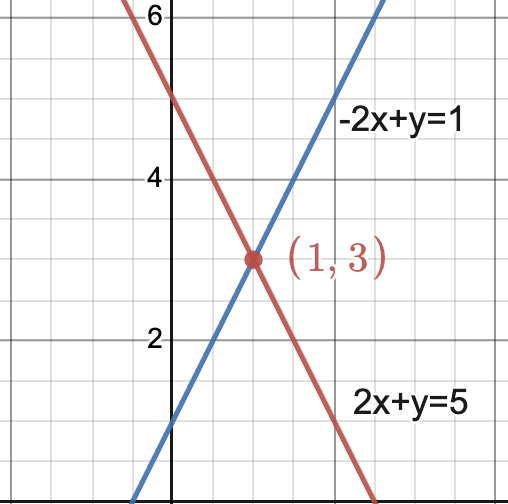
\includegraphics[width=4cm]{pre-op-1.png}
\end{center}
\par\noindent Let's suppose we applied the operation \( R_1 + R_2 = R_1 \):

\[
\left(\begin{array}{@{}cc|c@{}}
	-2 & 1 & 1 \\
	2 & 1 & 5
\end{array}\right)
\xrightarrow[]{R_1 + R_2 = R_1}
\left(\begin{array}{@{}cc|c@{}}
    0 & 2 & 6 \\
    2 & 1 & 5
\end{array}\right)
\]
\par \noindent Here is now the graph containing with the new \(R_1\), \(2y = 6\). 
\begin{center}
	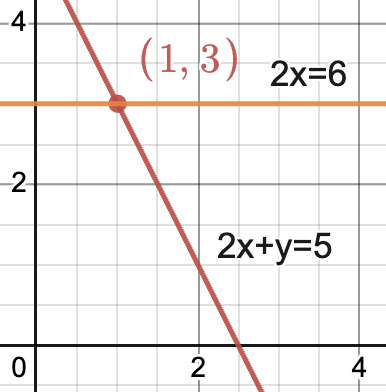
\includegraphics[width=4cm]{post-op-1.png}
\end{center}
\par \noindent Notice that the solution has not changed. 
\newline
\par\noindent Repeating this experiment with Example 2 leads us to the same conclusion. Suppose we 
applied the operation \(R_1 - R_2 = R_1 \) to the matrix in its starting state. On the graph below, the original \(R_1\) is the purple plane, and \(R_2\) is the red plane. The transformed \(R_1\)
is the mint plane. The formula for the transformed \(R_1\) is \(x-3y+z=-5\). The small red arrow is a vector representative of the solution line obtained in Example 2. We note that the solution line is shared by all three planes.
\newline
\begin{center}
	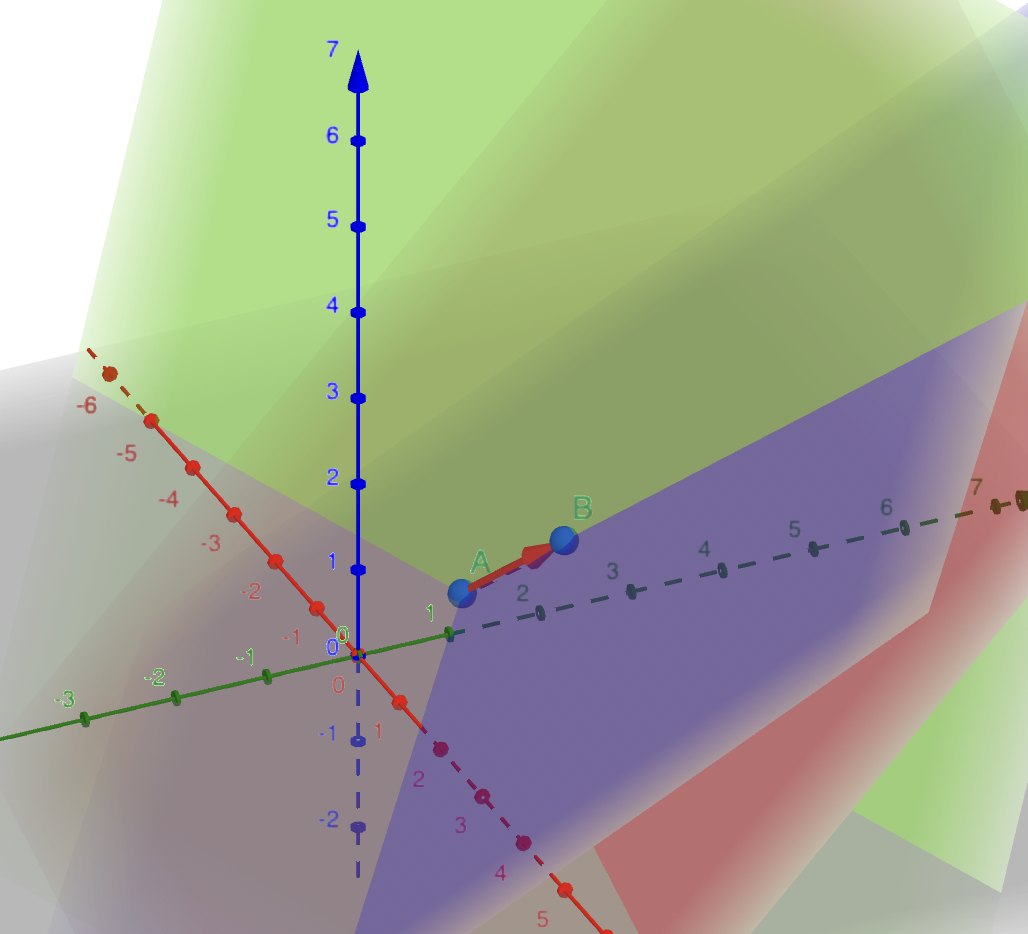
\includegraphics[width=4cm]{post-op-2.png}
\end{center}
\par \noindent  In fact, none of the elementary row operations will  change the solution to a linear system. On section 4, we'll show the intuition for why this is the case.

\pagebreak
\section {Elementary Matrices}
\par \noindent An elementary matrix is the result of applying an elementary row operation to an identity matrix. Our claim is that multiplying an elementary matrix by the original matrix is the same as applying the row operation directly to an original matrix.
\newline
\par\noindent Let's suppose we applied the operation \( R_1 - R_2 = R_1 \) to the matrix we started with in Example 2:
\[
\left(\begin{array}{@{}ccc|c@{}}
	2 & 3 & -4 & 3 \\
	1 & 6 & -5 & 8
\end{array}\right)
 \xrightarrow[]{R_1 - R_2 = R_1}
\left(\begin{array}{@{}ccc|c@{}}
	1 & -3 & 1 & -5 \\
	1 & 6 & -5 & 8
\end{array}\right)
\]
\par\noindent Let's see what happens when we apply the same operation to an identity matrix, then multiply the resulting elementary matrix by the original matrix. The identity matrix \(I_2\) is suitable in this case given the dimensions of the original array.
\[
\left(\begin{array}{@{}cc@{}}
	1 & 0 \\
	0 & 1 
\end{array}\right)
 \xrightarrow[]{R_1 - R_2 = R_1}
 \left(\begin{array}{@{}cc@{}}
	1 & -1 \\
	0 & 1 
\end{array}\right)
\]
\newline
\[
\left(\begin{array}{@{}cc@{}}
	1 & -1 \\
	0 & 1 
\end{array}\right)
\left(\begin{array}{@{}ccc|c@{}}
	2 & 3 & -4 & 3 \\
	1 & 6 & -5 & 8
\end{array}\right) = 
\left(\begin{array}{@{}ccc|c@{}}
	1 &- 3 & 1 & -5 \\
	1 & 6 & -5 & 8
\end{array}\right)
\]
\par \noindent We arrive at the same matrix regardless of the approach taken. We can show that this will always be the case for these dimensions regardless of the type of row operation.
\newline
\par \noindent \textbf{Exchanging two rows}: 
\[
 \left(\begin{array}{@{}cc@{}}
	1 & 0 \\
	0 & 1 
\end{array}\right)
 \xrightarrow[]{R_1 \Leftrightarrow R_2}
  \left(\begin{array}{@{}cc@{}}
	0 & 1 \\
	1 & 0 
\end{array}\right)
 \]
 \[
   \left(\begin{array}{@{}cc@{}}
	0 & 1 \\
	1 & 0 
\end{array}\right)
\left(\begin{array}{@{}ccc|c@{}}
	a & b & c & d \\
	e & f & g & h
\end{array}\right)=
\left(\begin{array}{@{}ccc|c@{}}
	e & f & g & h \\
	a & b & c & d
\end{array}\right)
\]
\par \noindent Notice that this is equivalent to applying \(R_1 \Leftrightarrow R_2\) directly to the original matrix:
\newline
\[
\left(\begin{array}{@{}ccc|c@{}}
	e & f & g & h \\
	a & b & c & d
\end{array}\right)
 \xrightarrow[]{R_1 \Leftrightarrow R_2}
 \left(\begin{array}{@{}ccc|c@{}}
	e & f & g & h \\
	a & b & c & d
\end{array}\right)
\]
\par \noindent \textbf{Multiply a row by a constant:}
\newline
\[
 \left(\begin{array}{@{}cc@{}}
	1 & 0 \\
	0 & 1 
\end{array}\right)
 \xrightarrow[]{kR_1 = R_1}
  \left(\begin{array}{@{}cc@{}}
	k & 0 \\
	0 & 1 
\end{array}\right)
 \]
 \[
   \left(\begin{array}{@{}cc@{}}
	k & 0 \\
	0 & 1 
\end{array}\right)
\left(\begin{array}{@{}ccc|c@{}}
	a & b & c & d \\
	e & f & g & h
\end{array}\right)=
\left(\begin{array}{@{}ccc|c@{}}
	ka & kb & kc & kd \\
	e & f & g & h
\end{array}\right)
\]
\par \noindent This is equivalent to applying \(kR_1 \Leftrightarrow R_1\) directly to the original matrix:
\[
\left(\begin{array}{@{}ccc|c@{}}
	a & b & c & d \\
	e & f & g & h
\end{array}\right)
 \xrightarrow[]{kR_1 = R_1}
\left(\begin{array}{@{}ccc|c@{}}
	ka & kb & kc & kd \\
	e & f & g & h
\end{array}\right)
\]
\par \noindent \textbf{Add a multiple of one row to another:}
\newline
\[
 \left(\begin{array}{@{}cc@{}}
	1 & 0 \\
	0 & 1 
\end{array}\right)
 \xrightarrow[]{R_1 + kR_2 = R_1}
  \left(\begin{array}{@{}cc@{}}
	1 & k \\
	0 & 1 
\end{array}\right)
 \]
  \[
   \left(\begin{array}{@{}cc@{}}
	1 & k \\
	0 & 1 
\end{array}\right)
\left(\begin{array}{@{}ccc|c@{}}
	a & b & c & d \\
	e & f & g & h
\end{array}\right)=
\left(\begin{array}{@{}ccc|c@{}}
	a + ke & b+kf & c + kg & d+kh \\
	e & f & g & h
\end{array}\right)
\]
\par \noindent This is equivalent to applying \(R_1 + kR_2 = R_1\) directly to the original matrix:
\[
\left(\begin{array}{@{}ccc|c@{}}
	a & b & c & d \\
	e & f & g & h
\end{array}\right)
 \xrightarrow[]{R_1 + kR_2 = R_1}
\left(\begin{array}{@{}ccc|c@{}}
	a + ke & b+kf & c + kg & d+kh \\
	e & f & g & h
\end{array}\right)
\]
\section{Why Solutions Don't Change}
\par \noindent We previously saw how elementary operations preserve the solution to a system, if it exists. In other words applying a row operation will not change the solution. Here is an insight into how this works, suppose we have a generic system of three equations and three variables with the equations on the left and the matrix on the right.
\newline
\newline
\begin{minipage}[c]{.5\linewidth}

\begin{flalign*}
ax + by + cz = d \\
ex + fy + gz = h \\
ix + jy + kz = l
\end{flalign*}
\end{minipage}
\begin{minipage}[c]{.5\linewidth}
\[
\left(\begin{array}{@{}ccc|c@{}}
	a & b & c & d \\
	e & f & g & h \\
	i & j & k & l
\end{array}\right)
\]\end{minipage}
\newline
\newline
\par \noindent \textbf{Exchanging two rows}: A silly proof for this is as follows - changing the order in which you plot the equations onto a graph does not affect the solution \smiley{}
\newline
\par \noindent \textbf{Multiply the row by a constant}: Suppose that we performed the operation \(kR_1 = R_1\). So we get the following: \(k(ax + by + cz) = kd \). Since d is just \(ax + by + cz \) we can do the following substitution:

\begin{flalign*}
k(ax + by + cz) = kd \\
k(ax + by + cz) = k(ax + by + cz)  \\
\cancel{k}(ax + by + cz) = \cancel{k}(ax + by + cz)  \\  
\end{flalign*}

\par\noindent We see that we ended up in a situation where if we cancel the k term on both sides we are left with the original, and therefore the solution to the system cannot change.
\newline
\par \noindent \textbf{Adding a multiple of one row to another}: Suppose we wanted to perform the operation \(R_1 + kR_2 = R_1\):

\begin{flalign*}
ax + by + cz + k(ex + fy + gz) = d + kh \\
ax + by + cz + k(ex + fy + gz) = d + k(ex + fy + gz) \\
ax + by + cz + \cancel{k(ex + fy + gz)} = d +\cancel{ k(ex + fy + gz)} \\
ax + by + cz = ax + by + cz
\end{flalign*}
\par \noindent We have once again arrived at a situation where there are cancellable terms that allow us to revert back to the original equation, and therefore the solution cannot change.
\newline
\par \noindent The key word here is \textbf{invertability}. There is some mechanism that allows us to undo the work performed by the row operation. This process can be visualized through matrices as well. We already saw how we could apply elementary row operations by using elementary matrices. 
\newline
\par\noindent Suppose our target matrix is \(A\) and we have an identity matrix of suitable dimensions \(I_n\) which has been transformed using a row operation to \(J\).  There exists an inverse matrix \(J^{    -1}\) such that \(J^{-1} \cdot J = I_n\). We therefore observe the following when applying an elementary row operation:

\begin{flalign*}
J^{-1} \cdot J \cdot A \\
= I_{n}  \cdot A \\
= A 
\end{flalign*}



\end{document}